%%%%%%%%%%%%%%%%%%%%%%%%%%%%%%%%%%%%%%%%%%%%%%
%                insertmeeting
% 1) Title (something creative & funny?)
% 2) Date (MM/DD/YYYY)
% 3) Location (ex. Hagerty High School)
% 4) People/Committees Present 
% 5) Picture 
% 6) Start Time & Stop Time (ex. 12:30AM to 4:30PM)
%%%%%%%%%%%%%%%%%%%%%%%%%%%%%%%%%%%%%%%%%%%%%%
\insertmeeting 
	{Fun Fundraising!} 
	{04/09/22} 
	{Hagerty High School}
	{James, Jensen, Nathan, Ritam}
	{Images/RobotPics/robot.jpg}
	{2:30 - 4:30}
	
\hhscommittee{Fundraising}
\noindent\hfil\rule{\textwidth}{.4pt}\hfil
\subsubsection*{Goals}
\begin{itemize}
    \item Raise money to pay for worlds

\end{itemize} 

\noindent\hfil\rule{\textwidth}{.4pt}\hfil

\subsubsection*{Accomplishments}
Today, we did our annual Hagerty Highschool Robotics car wash. At the car wash, we washed cars in order to raise money for the FTC Worlds Championship which we are going to in a couple weeks. We had a pretty great start as we were able to collect donations from student's parents as well as wash their cars. Unfortunately, as the day went on, less and less people were getting their car washed. That was until we had a large number of students from FTC Team 7592, Roarbots who is also in our local area. They were having a meeting and decided to send a couple people to get their car washed which was very helpful. As they were going to worlds as well, we were able to discuss changes in our robot and strategy for worlds. Overall, the car wash was a lot of fun and we raised \$717 from the experience. 

\begin{figure}[htp]
\centering
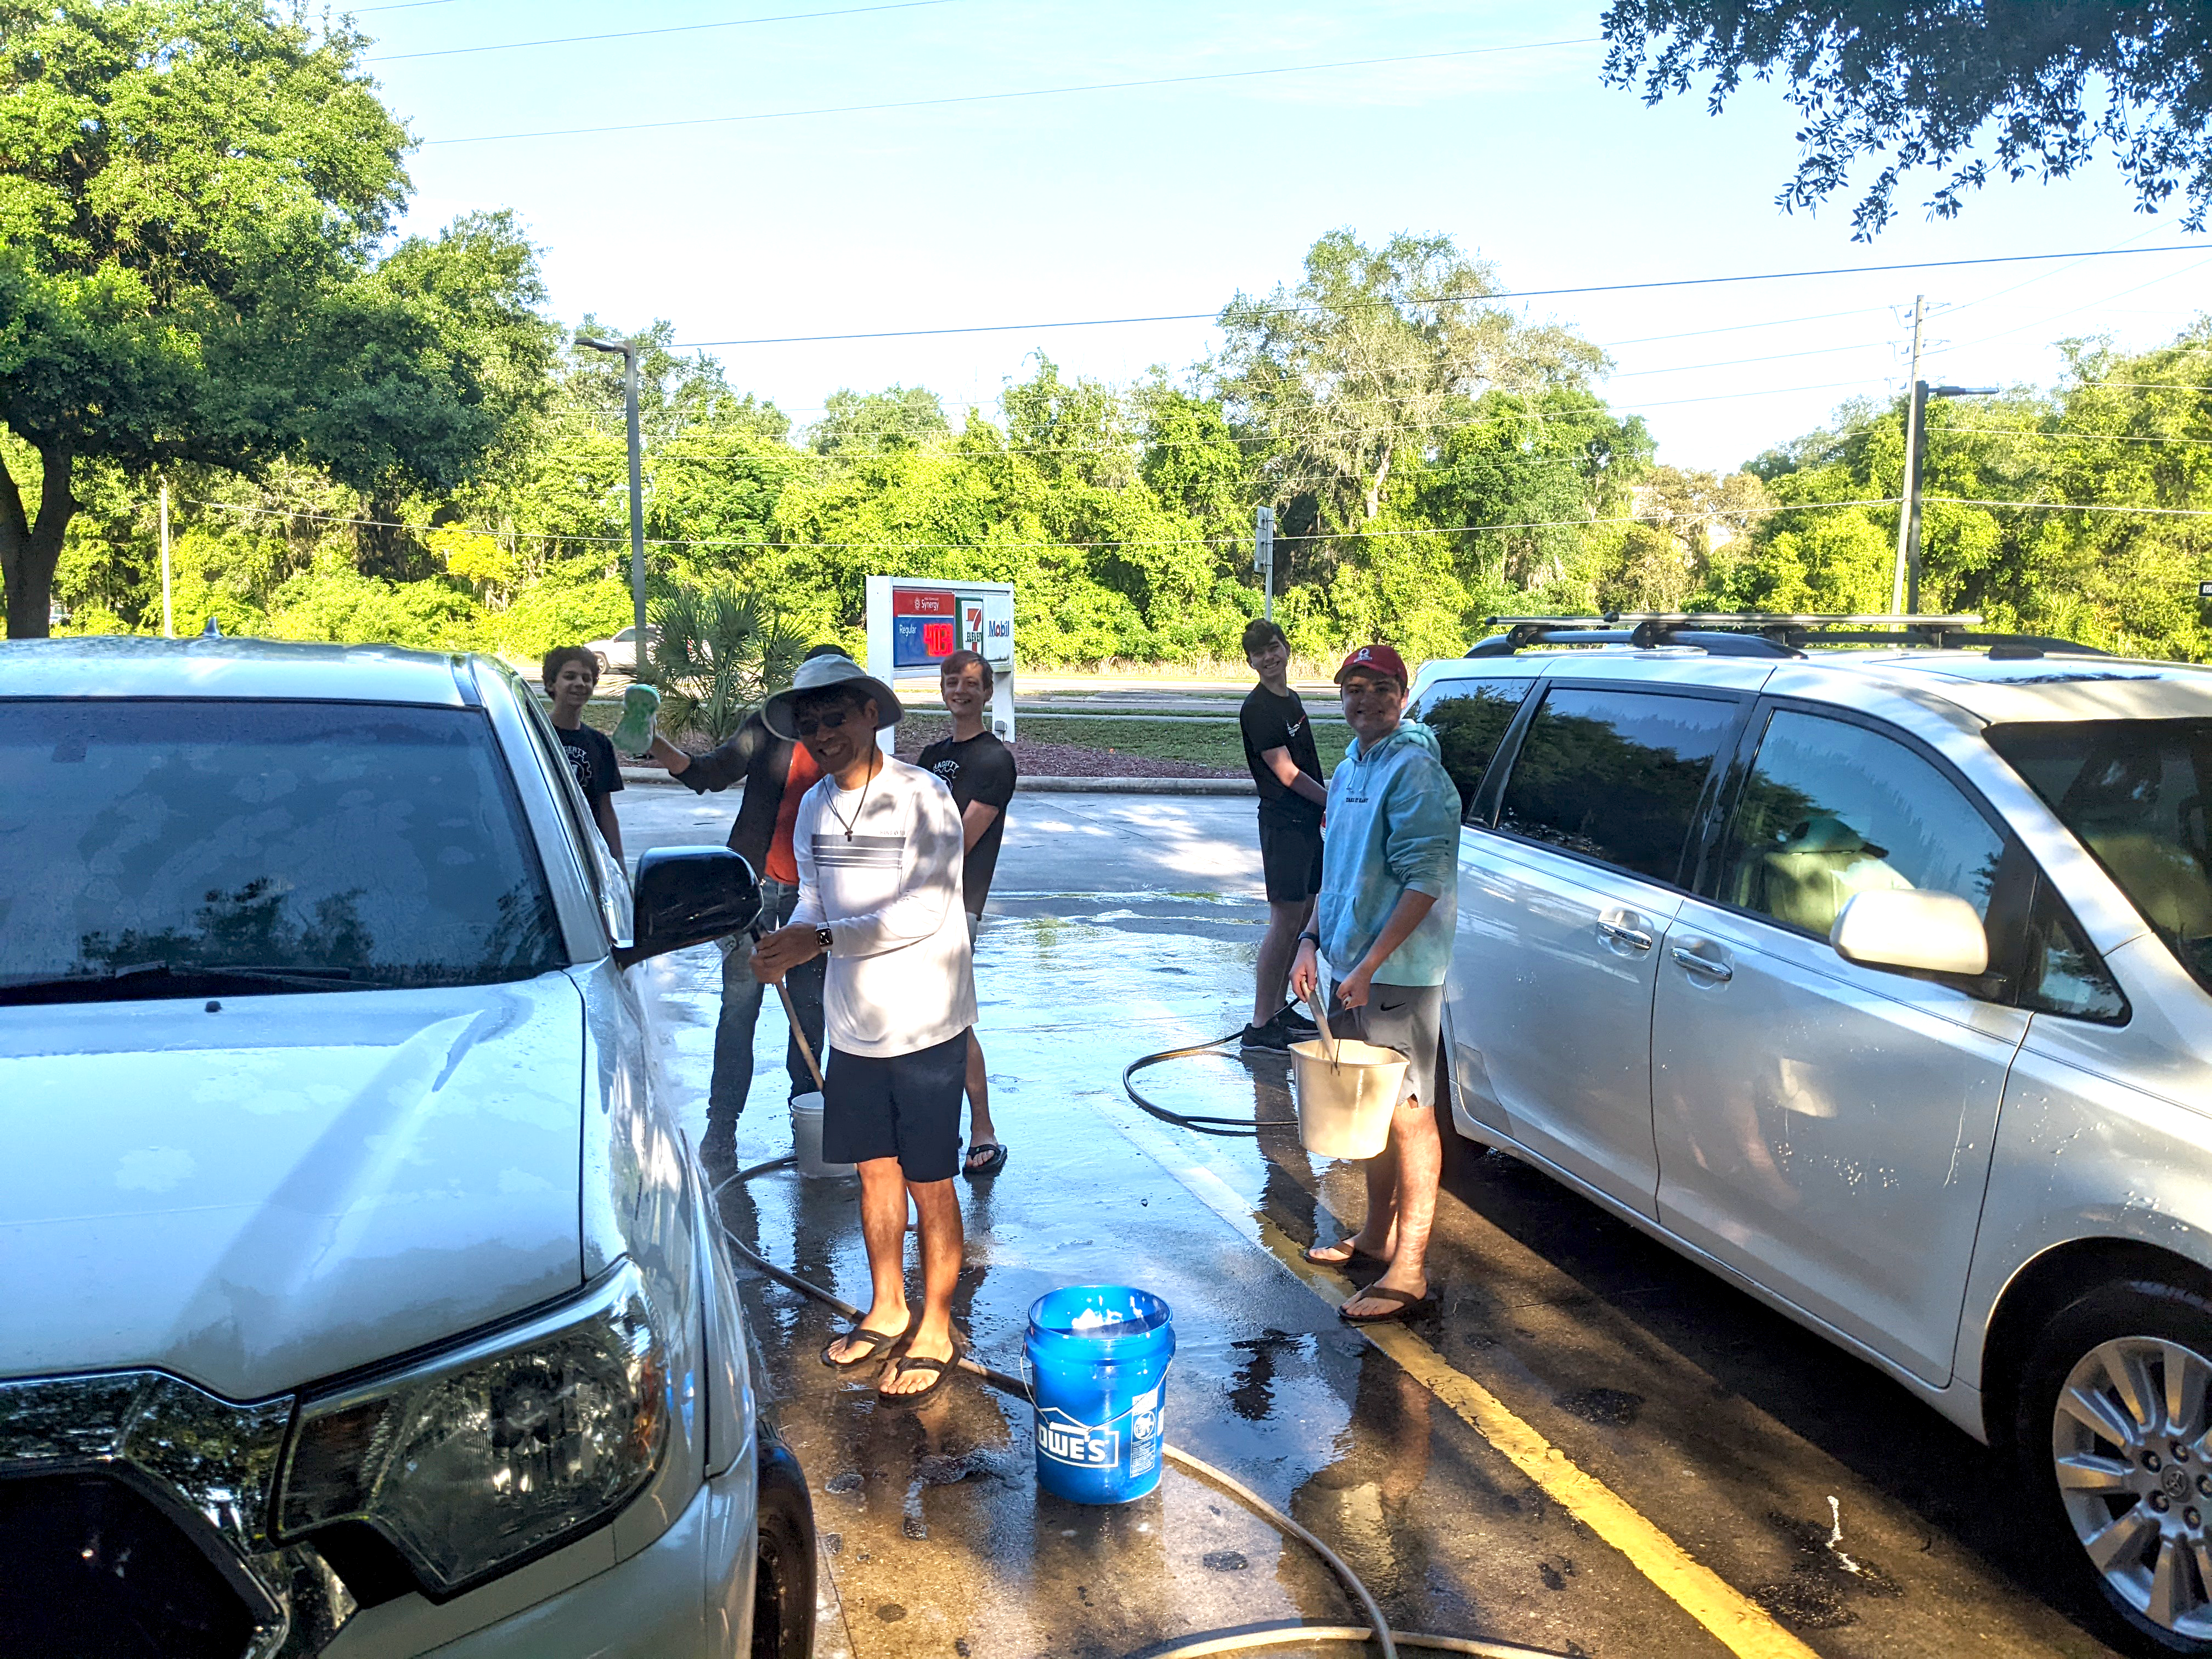
\includegraphics[width=0.95\textwidth, angle=0]{Meetings/April/04-09-22/04-09-22 1.png}
\caption{Car wash!}
\label{fig:041322_1}
\end{figure}


\whatsnext{
\begin{itemize}
    \item Finalizing everything for worlds
\end{itemize} 
}

